\documentclass[10pt]{article}

\usepackage{tabularx}
\usepackage[a4paper,margin=2.5cm, bottom=2.5cm]{geometry}
\usepackage{fancyhdr}
\usepackage{listings}
\usepackage{booktabs}
\usepackage{float}
\usepackage{subcaption}
% \usepackage{caption}
% \captionsetup{font=footnotesize}
\usepackage{graphicx}
\usepackage{amsmath}
\usepackage{amssymb}
\usepackage{amsthm}
\usepackage{array}
\usepackage[table]{xcolor}
\usepackage{pgfplots}
\pgfplotsset{compat=1.17}
\usepackage{pgfplotstable}
\usepackage{multirow}
\usepackage{tikz}
\usepackage[hidelinks]{hyperref}
\usepackage{titling}
\usepackage[polish]{babel} % Polish language support

\setlength{\headheight}{40pt}
\setlength{\parindent}{0pt}
\setlength{\parskip}{1ex}
\renewcommand{\headrulewidth}{0pt}

\pagestyle{fancy}
\fancyhead{}
\fancyhead[L]{
    \renewcommand{\arraystretch}{1.5}
    \begin{tabularx}{\textwidth}{|X|X|}
        \hline
        \bfseries Obliczenia inteligentne & \bfseries \thetitle \\
        \hline
    \end{tabularx}
}
\fancyfoot[C]{\thepage}

\renewcommand{\maketitle}{
    \thispagestyle{plain}
    \renewcommand{\arraystretch}{2}
    \vspace*{-8em}
    \footnotesize
    \begin{flushleft}
        \begin{tabularx}{\textwidth}{|X|X|}
            \hline
            \bfseries Obliczenia Inteligentne  & \bfseries \thetitle                           \\ \hline
            \multicolumn{2}{|l|}{
                \begin{tabular}[t]{@{}ll@{}} 
                    \textbf{Grupa:} Grupa 1
                    \hspace{4.5em}
                    \textbf{Dzień i czas:} Czwartek, 10:00
                    \hspace{4.5em}
                    \textbf{Rok akademicki:} 2023/24
                \end{tabular}
            } \\ \hline
            \multicolumn{2}{|l|}{
                \begin{tabular}[t]{@{}l@{\hspace{10em}}l@{}} 
                    \textbf{Imię i nazwisko:} \textsc{Jakub Pawlak} & \textbf{Imię i nazwisko:} \textsc{Magdalena Paku\l a} 
                \end{tabular}
            } \\
            \hline
        \end{tabularx}
    \end{flushleft}
    \renewcommand{\arraystretch}{1}
}


\title{Projekt 2 --- Zadanie 1}

\begin{document}
\maketitle
\normalsize
\section{Opis ekstrakcji cech --- Osoba 1}


\paragraph*{Analiza głównych składowych (PCA --- Principal Component Analysis)} to technika redukcji wymiarowości danych powszechnie stosowana do ekstrakcji cech. W kontekście zestawu danych MNIST, PCA może być stosowana do zmniejszenia wymiarowości danych obrazowych, zachowując przy tym większość ich wariancji.

Metoda ekstrakcji cech PCA przekształca dane obrazowe o wysokiej wymiarowości do przestrzeni o niższej wymiarowości, identyfikując główne składowe danych. Te główne składowe to ortogonalne kierunki w przestrzeni cech, które przechwytują maksymalną wariancję danych.

W naszej implementacji PCA jest stosowana do spłaszczenia każdego obrazu o rozmiarze $28\times28$ pikseli do wektora o wymiarach 784. Następnie otrzymane wektory są przekształcane do przestrzeni o niższej wymiarowości, zwykle dwóch wymiarów w celu wizualizacji.

\begin{figure}[h]
    \centering
    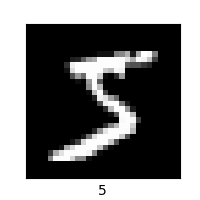
\includegraphics[width=0.3\textwidth]{img/MNIST_1_cyfra}
    \caption{Przykładowy obraz cyfry ``5'' z zestawu danych MNIST.}
\end{figure}

Poniżej znajdują się wygenerowane cechy dla powyższego obrazu ``5'' za pomocą PCA\@:
\begin{table}[H]
    \centering
    \begin{tabular}{|c|c|c|}
        \toprule
        \textbf{Piksel} & \textbf{PCA cecha 1} & \textbf{PCA cecha 2} \\
        \midrule
        1               & -248.0374            & 36.2011              \\
        2               & -248.0374            & 36.2011              \\
        \ldots          & \ldots               & \ldots               \\
        28              & -248.0374            & 36.2011              \\
        \bottomrule
    \end{tabular}
    \caption{Wartości wygenerowanych cech za pomocą PCA dla obrazu ``5''.}
\end{table}


\paragraph*{Binary Patterns (LBP)} to deskryptor tekstury używany do ekstrakcji cech w obrazach. W kontekście zestawu danych MNIST, LBP może być stosowany do wydobycia cech tekstury z obrazów.

Metoda ekstrakcji cech LBP działa przez podzielenie obrazu na małe obszary i porównanie każdego piksela z otaczającymi go pikselami. Na podstawie tych porównań dla każdego piksela tworzony jest wzorzec binarny. Poprzez zliczanie wystąpień różnych wzorców binarnych konstruowany jest histogram reprezentujący cechy tekstury obrazu.

Poniżej znajdują się wygenerowane cechy dla powyższego obrazu ``5'' za pomocą LBP\@:

\begin{table}[H]
    \centering
    \begin{tabular}{|c|c|}
        \toprule
        \textbf{LBP cecha} & \textbf{Wartość} \\
        \midrule
        1                  & 3.0              \\
        2                  & 11.0             \\
        3                  & 6.0              \\
        4                  & 32.0             \\
        5                  & 48.0             \\
        6                  & 34.0             \\
        7                  & 2.0              \\
        8                  & 4.0              \\
        9                  & 618.0            \\
        10                 & 26.0             \\
        \bottomrule
    \end{tabular}
    \caption{Wartości wygenerowanych cech za pomocą LBP dla obrazu ``5''.}
\end{table}

\pagebreak

\section{Wyniki eksperymentu --- Osoba 1}
\pagebreak

\section{Opis ekstrakcji cech --- Osoba 2}

\paragraph{Histogram of Oriented Gradients (HOG)} to metoda ekstrakcji cech używana w przetwarzaniu obrazu.
Opiera się ona na zliczaniu gradientów zorientowanych w tym samym kierunku, w określonych fragmentach obrazu.
Deskryptor HOG opisuje kształt obiektu na obrazie, więc bardzo dobrze nadaje się do zadania rozpoznawania cyfr, ponieważ następuje ono właśnie na podstawie kształtu.

Alorytm najpierw dzieli obraz na komórki o określonym rozmiarze. W przypadku zbioru MNIST użyto komórek $14\times14$, uzyskując podział całego obrazu na 4 komórki.
W każdej komórce, oblicza się dla każdego piksela lokalny gradient.
Następnie, wewnątrz każdej komórki zlicza się gradienty w określonych kierunkach i tworzy się z nich histogram.
Aby umożliwić wykrycie linii zarówno ortogonalnych jak i ukośnych, liczba kierunków została ustawiona na 9.
W celu poprawy jakości, wartości gradientów są dodatkowo normalizowane w większych grupach.
W tym przypadku, użyto grup o rozmiarze $2\times2$ komórek, co odpowiada całemu obrazowi.

Cały obraz zostaje zatem opisany za pomocą 4 komórek, każda zawierająca wartości dla 9 kierunków.
W ten sposób obraz $28\times28$ zredukowano do 36-elementowego wektora.

\begin{figure}[H]\centering
    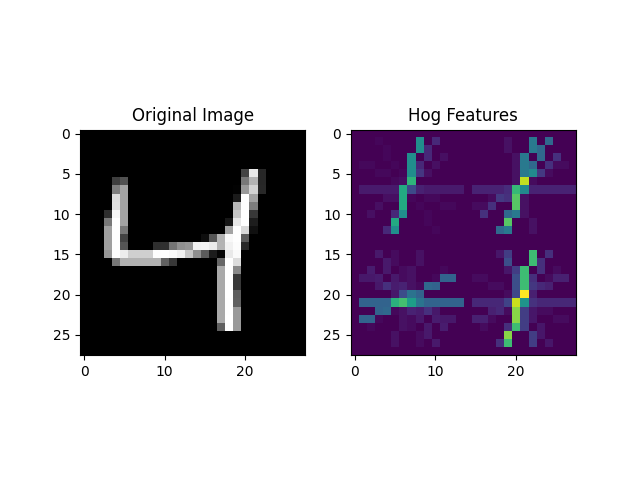
\includegraphics[width=.32\linewidth]{img/hog_vis/4.png}
    \hfill
    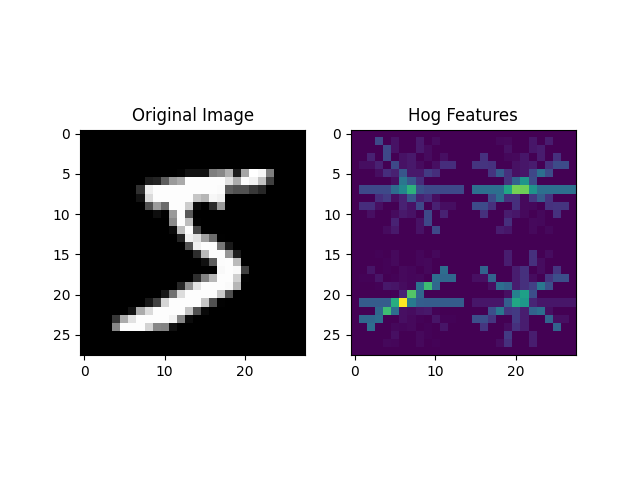
\includegraphics[width=.32\linewidth]{img/hog_vis/5.png}
    \hfill
    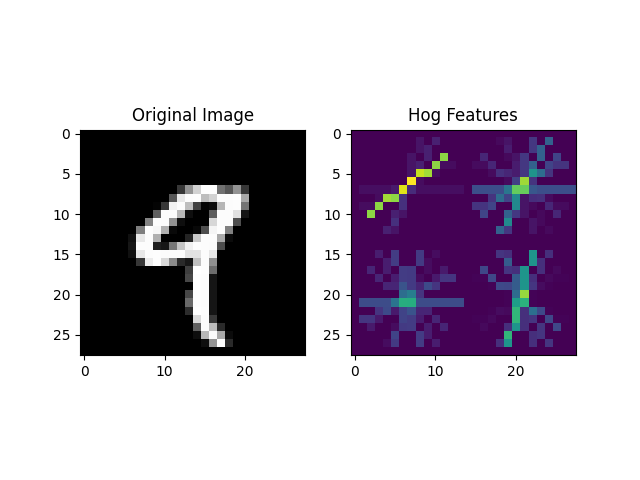
\includegraphics[width=.32\linewidth]{img/hog_vis/9.png}
    \caption{Przykłady ekstrakcji cech metodą HOG}
\end{figure}




\paragraph{t-Distributed Stochastic Neighbor Embedding (t-SNE)} jest stochastyczną metodą redukcji wymiarów, często wykorzystywaną przy tworzeniu wizualizacji.


Próbuje ona rozłożyć punkty w przestrzeni docelowej zachowując lokalnych sąsiadów z przestrzeni źródłowej.
Metoda ta bada odległości między punktami w przestrzeni źródłowej i przypisuje im rozkład prawdopodobieństwa w opraciu o rozkład standardowy.
Następnie wybiera (losowo lub przez PCA) rozkład punktów w przestrzeni docelowej i analizuje ich odległości, przypisując im prawdopodobieństwa oparte o rozkład Cauchy'ego.
Następnie za pomocą metody minimalizacji gradientu stara się zminimalizować różnicę pomiędzy rozkładami w przestrzeni źródłowej i docelowej.

\begin{figure}[H]\centering
    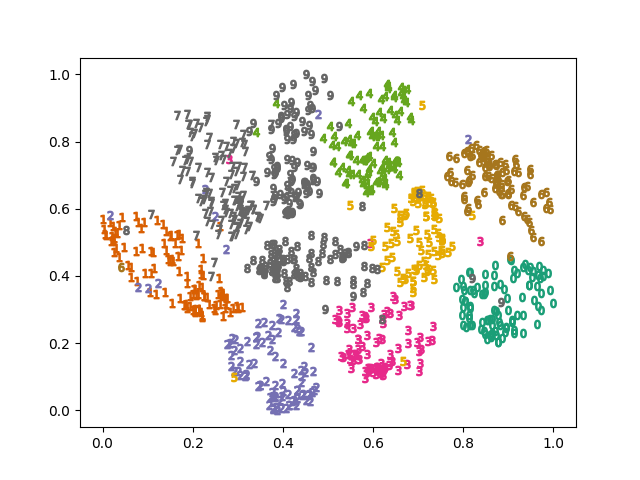
\includegraphics[width=.6\linewidth]{img/tsne_embedding.png}
    \caption{Wizualicacja docelowej przestrzeni t-SNE}\label{fig:tsne-embed}
\end{figure}

\pagebreak

\section{Wyniki eksperymentu --- Osoba 2}

Dla ekstrakcji cech w celu oceny separowalności wytrenowano sieć z małą ilością epok i oceniono macierz pomyłek, która znajduje się na rys~\ref{fig:hog-bad-cm}.

\begin{figure}[H]\centering
    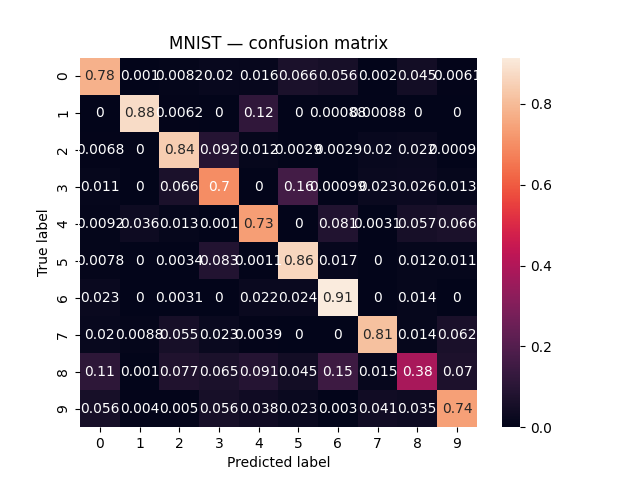
\includegraphics[width=.3\linewidth]{img/mnist_hog_bad_cm.png}
    \caption{Macierz pomyłek na słabo wytrenowanej sieci (ekstakcja HOG)}\label{fig:hog-bad-cm}
\end{figure}

Zauważyć można, że najgorzej model radzi sobie z rozpoznawaniem cyfr 8,3,4, 9 i 0.
Cyfra 8 bardzo często uznawana jest za 0,2,3,4 lub 6.
Często mylone są również 3 i 5.
Wynika to z faktu, że algorytm HOG wewnątrz komórek uzwględnia tylko ilość gradientów, a nie ich położenie względem siebie.
Dla przykładu, na rys.~\ref{fig:hig-similar} przedstawiono różne cyfry, które po ekstrakcji cech wyglądają podobnie.
Tak oto przedstawione cyfry 3 oraz 5 obie posiadają w prawej górnej ćwiartce linię ukośną i poziomą.
W cyfrze 3 linia pozioma idzie w prawo, a w cyfrze 5 --- w lewo, natomiast dla algorytmu HOG nie ma to znaczenia, ponieważ obie linie znajdują się w tej samej komórce.
Podobnie z cyframi 7 i 9, różniącymi się jedynie poziomym domknięciem, co jednak nie znajduje odzwierciedlenia w deskryprorze HOG, ponieważ pozioma linia już występuje gdzie indziej w tej samej ćwiartce.


\begin{figure}[H]\centering
    \begin{subfigure}[t]{.2\textwidth}
        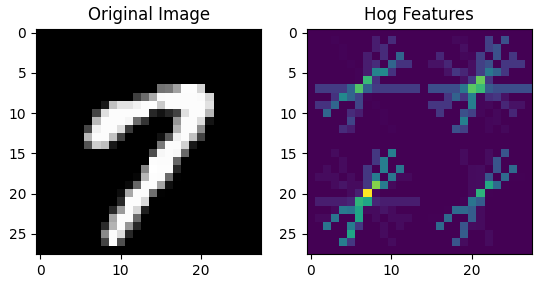
\includegraphics[width=\linewidth]{img/hog_similar/7.png}
        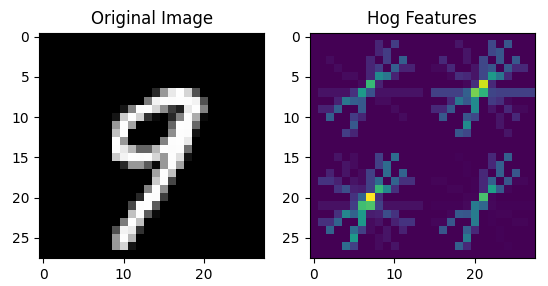
\includegraphics[width=\linewidth]{img/hog_similar/9.png}
        \caption{Podobne cechy dla różnych cyfr: 7 i 9}
    \end{subfigure}
    \hspace{.1\textwidth}
    \begin{subfigure}[t]{.2\textwidth}
        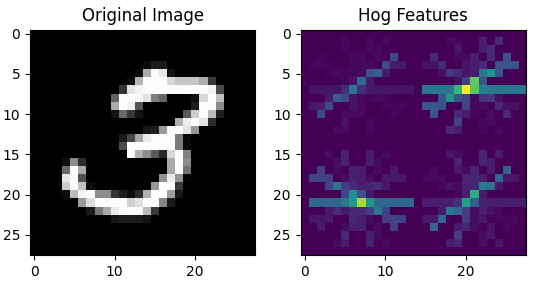
\includegraphics[width=\linewidth]{img/hog_similar/3.png}
        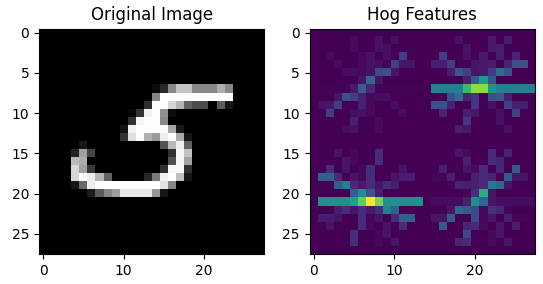
\includegraphics[width=\linewidth]{img/hog_similar/5.png}
        \caption{Podobne cechy dla różnych cyfr: 3 i 5}
    \end{subfigure}
    \caption{Różne cyfry, które posiadają podobne cechy}\label{fig:hig-similar}
\end{figure}

W metodzie t-SNE można ocenić separowalność wizualnie, na podstawie rys.~\ref{fig:tsne-embed},
jak również diagramu Woronoja na rys.~\ref{fig:tsne-voronoi}.
Od razu widać, że poszczególne klasy są separowalne, choć zdarzają się pola do pomyłek, zwłascze przy cyfrach 3,5 i 8, oraz 7,9 i 4.


\begin{figure}[H]\centering
    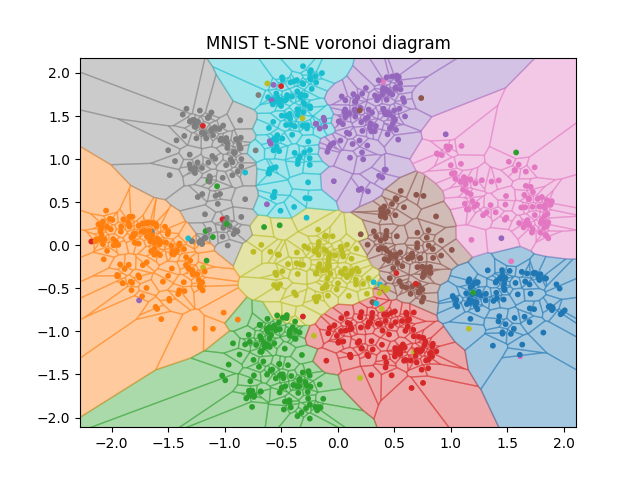
\includegraphics[width=.4\linewidth]{img/mnist_tsne_voronoi.png}
    \caption{Diagram Woronoja dla zbioru po przekształceniu t-SNE}\label{fig:tsne-voronoi}
\end{figure}


\pagebreak
\section{Wybór optymalnego modelu}

Podczas eksperymentów przeprowadzonych w ramach pierwszego projektu dało się zauważyć, że w miarę zwiększania
liczby neuronów w warstwie ukrytej, skuteczność ewentualnie ulegała wypłaszczeniu.
W takim przypadku, zwiększanie liczby neuronów skutkowałoby jedynie utrudnieniem obliczeń, bez pozytywnego efektu na skuteczności modelu.
Optymalnym modelem jest zatem taki, który maksymalizuje dokładność przy jednoczesnym minimalizowaniu ilości neuronów.

Przeprowadzone eksperymenty nie dostarczyły natomiast jednoznacznego sposobu, aby a priori określić najlepszą liczbę neuronów w warstwie ukrytej.
Wybór optymalnego modelu został dokonany poprzez coraz dokładnejsze przeszukiwanie przestrzeni liczb naturalnych, podobne w zasadzie działania do algorytmu \emph{binary search}.
Różne wartości liczby neuronów były poddawane przyśpieszonemu procesowi uczenia (na mniejszym zbiorze danych oraz mniejszą ilością epok), którego to wyniki pozwalały na oszacowanie, które wartości są najbardziej obiecujące.
Następnie wybierane zostały kolejne ilości neuronów do sprawdzenia --- tym razem z sąsiedztwa najlepiej spisujących się w poprzedniej iteracji.
Proces powtarzano, aż do znalezienia lokalnego maksimum skutecznośći.

Metoda ta pozwoliła uzyskać satysfakcjonujące wyniki, jendak wskazać należy, że jesteśmy świadomi iż nie daje ona gwarancji, że wybrany model jest globalnie optymalny.

\pagebreak

\section{Wyniki klasyfikacji dla pierwszego sposobu ekstrakcji cech}

\begin{figure}[H]
    \centering
    \begin{subfigure}[t]{0.3\textwidth}
        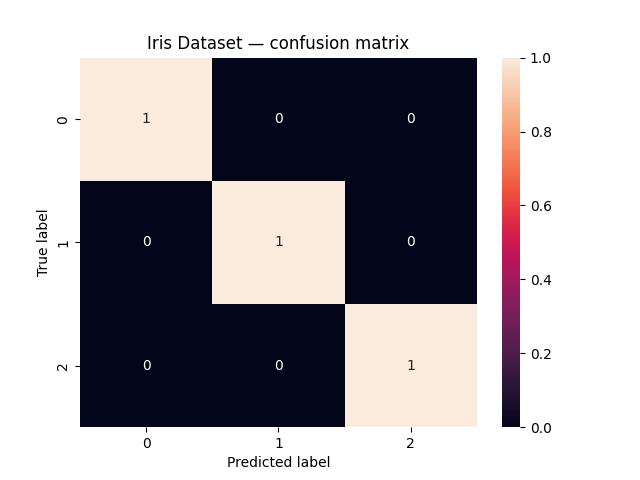
\includegraphics[width=\linewidth]{img/iris_cm.png}
        \caption{Zbior Iris}
    \end{subfigure}
    \hfill
    \begin{subfigure}[t]{0.3\textwidth}
        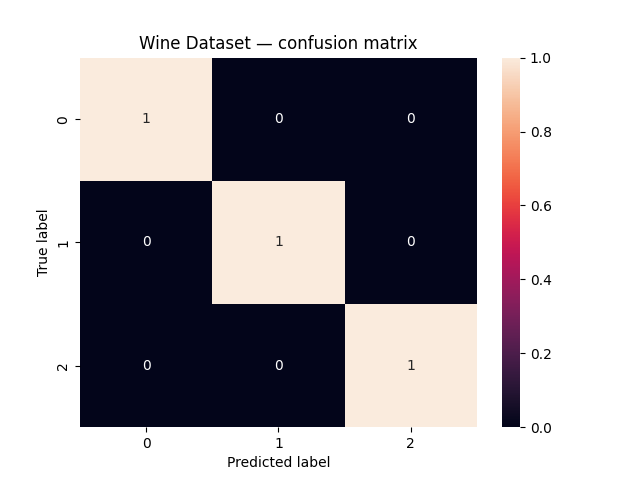
\includegraphics[width=\linewidth]{img/wine_cm.png}
        \caption{Zbior Wine}
    \end{subfigure}
    \hfill
    \begin{subfigure}[t]{0.3\textwidth}
        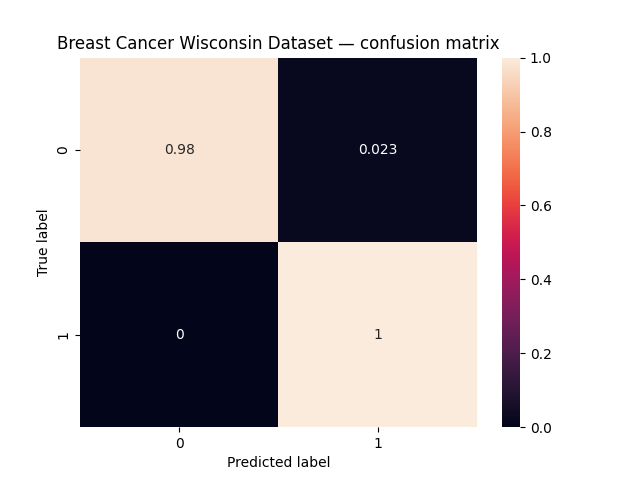
\includegraphics[width=\linewidth]{img/cancer_cm.png}
        \caption{Zbior Breast Cancer Wisconsin}
    \end{subfigure}
    \begin{subfigure}[t]{0.5\textwidth}
        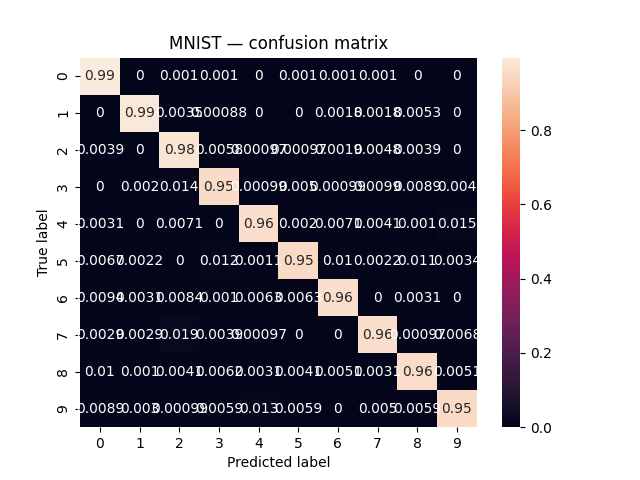
\includegraphics[width=\linewidth]{img/mnist_flat_cm.png}
        \caption{Zbior MNIST}
    \end{subfigure}
    \caption{Wyniki klasyfikacji dla 1 sposobu ekstrakcji cech}
\end{figure}

\begin{table}[H]\centering
    \begin{tabular}{lc}
        \toprule
        Zbiór danych            & Wartość Accuracy \\
        \midrule
        Iris                    & 93.33\%          \\
        Wine                    & 100\%            \\
        Breast Cancer Wisconsin & 99.12\%          \\
        MNIST                   & 97.16\%          \\
        \bottomrule
    \end{tabular}
    \caption{Wartości accuracy wytrenowanego modelu}
\end{table}

\pagebreak

\section{Wyniki klasyfikacji --- Osoba 1}
\pagebreak

\section{Wyniki klasyfikacji --- Osoba 2}

\subsection{HOG}

Wyniki klasyfikacji z metodą HOG przedstawiono na rys.~\ref{fig:hog-cm}.
Widać znaczą poprawę w stosunku do wstępnych oczekiwań, choć tak jak przewidziano, z cyframi 2,3,7,8,9 model radzi sobie słabiej niż z resztą.
Tak jak przewidywano, często mylone są cyfry pary (2,3), (3,5), (7,9), (8,6), (8,9).
Ogólna wartość accuracy osiągnęła 89.21\%.

\begin{figure}[H]
    \centering
    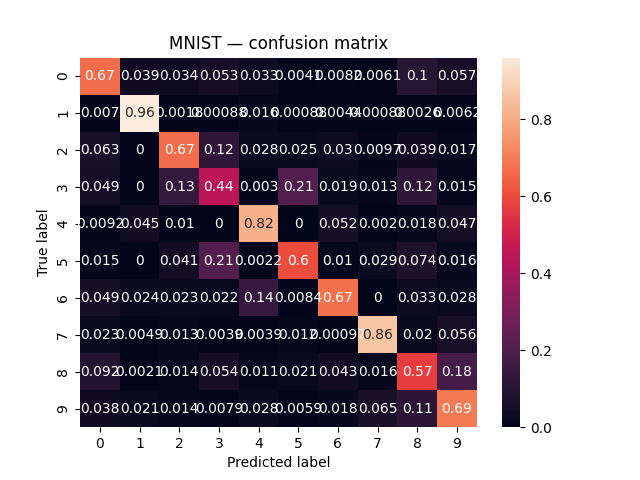
\includegraphics[width=.6\linewidth]{img/mnist_hog_cm.png}
    \caption{Wyniki klasyfikacji dla ekstrakcji cech metodą HOG (Accuracy: 89.21\%.)}\label{fig:hog-cm}
\end{figure}

\subsection{t-SNE}

Na rys.~\ref{fig:tsne-cm} przestawiono macierz pomyłek oraz przebieg granicy decyzyjnej.
Model poradził sobie bardzo dobrze, jednak można zauważyć drobne pomyłki.
Zgodnie z przewidywaniami, 4 i 7 były często uznawane za 9, jak również mylone były cyfry z grupy 3,5,8.
Pomimo mniejszej liczby cech, model osiągnął lepszą niż w poprzedniej metodzie wartość accuracy wynoszącą 95.67\%.
Wskazać jednak należy istotną wadę tej metody, mianowicie t-SNE operuje na całym zbiorze danych, więc użycie tej metody 
ekstrakcji cech nie będzie można zastosować w przypadku pojawnienia się nowych danych.

\begin{figure}[H]
    \centering
    \begin{subfigure}[t]{.5\textwidth}\centering
        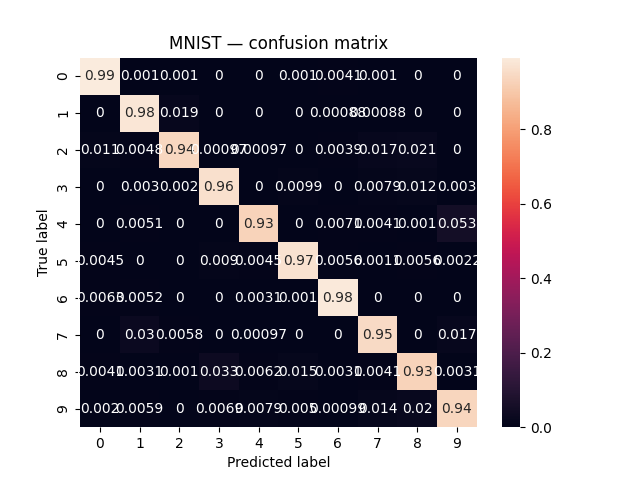
\includegraphics[width=\linewidth]{img/mnist_tsne_cm.png}
        \caption{Macierz pomyłek}\label{fig:tsne-cm}
    \end{subfigure}
    \hspace{-3em}
    \begin{subfigure}[t]{.5\textwidth}\centering
        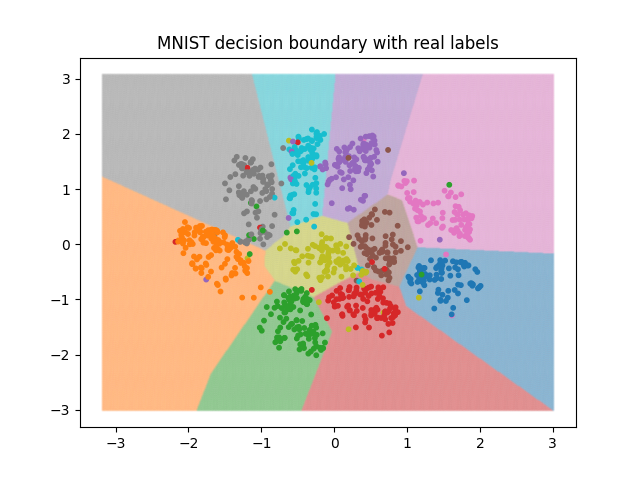
\includegraphics[width=\linewidth]{img/mnist_tsne_db.png}
        \caption{Granice decyzyjne}\label{fig:tsne-db}
    \end{subfigure}
    \caption{Wyniki klasyfikacji dla ekstrakcji cech metodą t-SNE (Accuracy: 95.67\%)}
\end{figure}






\end{document}